\documentclass[10pt,a4paper]{article}
\usepackage[margin=2.2cm]{geometry}
\usepackage[T1]{fontenc}
\usepackage{lmodern}
\usepackage{amsmath,booktabs,array,longtable,enumitem,xcolor}
\usepackage[hidelinks]{hyperref}
\usepackage{listings}
\usepackage{graphicx}
\lstset{basicstyle=\ttfamily\small,columns=fullflexible,frame=single,
  showstringspaces=false,keepspaces=true,framesep=4pt,xleftmargin=6pt,xrightmargin=6pt,breaklines=true}
\newcommand{\kw}[1]{\texttt{#1}}
\setlength{\parindent}{0pt}\setlength{\parskip}{5pt}
\title{Ion energy and angular distributions from a SOMAFOAM run\\[4pt]
\large Running the cross sections $\rightarrow$ fluid $\rightarrow$ ion
tracking chain for other conditions}
\date{}
\begin{document}
\sloppy
\maketitle
\vspace{-1.2cm}

\section{What the chain does}

Three programs are run one after the other; each uses the output of the one
before.

\begin{center}
\begin{tabular}{@{}ll>{\raggedright\arraybackslash}p{9.3cm}@{}}
\toprule
Step & Program & Input $\rightarrow$ output \\
\midrule
1 & \kw{electronBoltzmann} & electron cross sections $\rightarrow$ electron
  mobility, diffusion coefficient and rate coefficients against the electron
  temperature \\
2 & \kw{somaFoam} & those tables, the ion mobility and the discharge
  conditions $\rightarrow$ densities, electron temperature and the electric
  field over the RF period \\
3 & \kw{ionTracker} & the electric field at a number of phases of one period
  and ion--neutral cross sections $\rightarrow$ energy and angular
  distributions of the ions at the electrodes \\
\bottomrule
\end{tabular}
\end{center}

The worked case is \kw{examples/plasma/HeliumIonDistribution}: a
one-dimensional helium discharge, 6.7\,cm gap, $3.21\times10^{22}$\,m$^{-3}$
(133\,Pa) at 300\,K, 120\,V at 13.56\,MHz, absorbing electrodes without
secondary emission. These are the conditions of case 4 of Turner
\emph{et al.}, Phys.\ Plasmas \textbf{20}, 013507 (2013), a benchmark
for particle-in-cell codes. After \kw{source <SOMAFOAM>/etc/bashrc},
\kw{./Allrun} runs all the steps (about seven hours on one core, nearly all
in step 2) and \kw{./caseClean} removes the results. Sections 3 to 5 follow
that script, section 6 says what to change for other conditions, and
section 8 gives the results of the example.

\section{Files of the case}

\begin{longtable}{@{}>{\raggedright\arraybackslash}p{6.1cm}>{\raggedright\arraybackslash}p{9.7cm}@{}}
\toprule
File & Contents \\
\midrule
\kw{constant/He\_electron.txt} & electron--neutral cross sections, LXCat
  format \\
\kw{constant/He+\_He.txt} & ion--neutral cross sections, LXCat format
  (blocks \kw{ISOTROPIC} and \kw{BACKSCAT}) \\
\kw{constant/mu\_Hep1} & ion mobility: $E/N$ [Td] and $\mu N$
  [1/(V\,m\,s)] \\
\kw{system/boltzmannDict} & step 1: gas, range of $E/N$, tables to write \\
\kw{constant/plasmaProperties} & species, transport models, flux scheme;
  \kw{electronBoltzmann yes;} makes \kw{somaFoam} run step 1 itself \\
\kw{constant/reactions} & reactions, the table of each and its energy loss
  [J] \\
\kw{constant/thermoProperties} & species and their masses \\
\kw{constant/polyMesh/blockMeshDict} & gap and number of cells \\
\kw{0/He}, \kw{0/p}, \kw{0/T} & gas density [1/m$^3$], pressure [Pa],
  temperature [K] \\
\kw{0/Phi} & voltage amplitude and frequency of the driven electrode \\
\kw{0/electron}, \kw{0/Hep1}, \kw{0/Te} & initial values and wall conditions
  (secondary emission coefficient \kw{seec}) \\
\kw{system/setExpressionFieldsDict} & initial density profile \\
\kw{system/controlDict} & time step, run length, output \\
\kw{system/ionTrackerDict} & step 3 \\
\kw{Allrun}, \kw{caseClean} & run all the steps; remove the results \\
\kw{warpx/inputs} & input of the particle-in-cell code WarpX for the same
  case (section 8) \\
\midrule
\multicolumn{2}{@{}l}{Written by step 1:} \\
\kw{constant/mu\_electron}, \kw{D\_electron} & electron mobility and
  diffusion coefficient times the gas density, against $T_e$ [K] \\
\kw{constant/reaction\_elastic}, \kw{\_exc1}, \kw{\_exc2}, \kw{\_ion} &
  rate coefficients against $T_e$ [K] \\
\kw{constant/boltzmann/} & all the results against $E/N$, and the energy
  distributions \\
\bottomrule
\end{longtable}

\section{Step 1: electron tables}

\begin{lstlisting}
file            "constant/He_electron.txt";
gases           ((He 1.0));          // (target fraction) ...
gasTemperature  300;
reducedField    { min 0.001; max 300; n 111; }     // Td
nEnergyCells    600;
tables
{
    mobility    "constant/mu_electron";
    diffusion   "constant/D_electron";
    rates       (("constant/reaction_elastic" 0) ("constant/reaction_exc1" 1)
                 ("constant/reaction_exc2" 2) ("constant/reaction_ion" 3));
}
\end{lstlisting}

The numbers in \kw{rates} are the positions of the processes in the list that
\kw{electronBoltzmann} prints (the order of the cross-section file). The file
names are those used in \kw{constant/reactions}.

\begin{itemize}[leftmargin=1.4em,itemsep=1pt]
\item Run it by hand with \kw{electronBoltzmann}, or leave
  \kw{electronBoltzmann yes;} in \kw{constant/plasmaProperties}.
\item The tables are against the electron temperature
  $T_e=\tfrac23\langle\varepsilon\rangle/k_B$ and do not depend on the
  pressure: they need to be made again only if the gas, the mixture or the gas
  temperature changes.
\item The range of $E/N$ must give electron temperatures that cover those of
  the discharge. \kw{constant/boltzmann/transport.dat} lists $T_e$ for every
  $E/N$. Outside the table the fluid solver uses the end value.
\item \kw{method monteCarlo;} replaces the two-term solution by a Monte Carlo
  swarm simulation. Use it to check the two-term tables where ionisation is
  strong (above roughly 100\,Td in argon). In helium the two-term solution
  has no steady state above a few hundred Td; the example stops at 300\,Td.
\end{itemize}

\section{Step 2: fluid solution}

\begin{lstlisting}
blockMesh
setExpressionFields
somaFoam
\end{lstlisting}

\textbf{Run length.} The densities settle on the ambipolar diffusion time,
which is thousands of RF periods at this pressure. The example starts from a
cosine profile near the expected density (\kw{setExpressionFieldsDict}) and
runs 6000 periods of 250 time steps; the mid-plane density is steady to
0.1\,\% after about 4000. Check that the run has settled before step 3:

\begin{lstlisting}
<SOMAFOAM>/postprocessing/plot_1d.py . --fields N_Hep1Mean TeMean --history
\end{lstlisting}

\textbf{Phase-resolved output.} \kw{ionTracker} needs the fields \kw{E},
\kw{J\_<ion>}, the ion and electron densities, the gas density and \kw{T} at
\kw{nPhases} equally spaced times of one period. \kw{Allrun} continues the
run for one period with

\begin{lstlisting}
startFrom       latestTime;
endTime         <latest time + one period>;
writeControl    timeStep;
writeInterval   5;          // 250 steps per period / 5 = 50 phases
\end{lstlisting}

The number of time steps per period must be a multiple of \kw{nPhases}.
\kw{E} and \kw{J\_<ion>} are written because they are listed in
\kw{objectNames} of the \kw{dumpObjects} function in \kw{system/controlDict}.

\section{Step 3: ion distributions}

\begin{lstlisting}
ion             Hep1;
ionMass         4.002602;           // amu
charge          1;
electricField   E;
gasDensity      He;
gasTemperature  T;
startTime       4.4247788e-04;      // first of the nPhases outputs (set by Allrun)
period          7.3746312684e-08;   // 1/13.56 MHz
nPhases         50;
source          fluxDivergence;     // needs J_Hep1 in the outputs
launch          sheath;             // track the sheaths only
nParticles      100000;
nThreads        4;
patches         (electrode ground);
crossSections   LXCat;
file            "constant/He+_He.txt";
energyFrame     centreOfMass;       // frame of the energies of the file
maxCollisionEnergy 300;             // eV
writeParticles  yes;
\end{lstlisting}

Output in \kw{ionTracker/}, for each patch: \kw{<patch>\_energy.dat},
\kw{<patch>\_angle.dat}, \kw{<patch>\_energyAngle.dat} (the joint
distribution) and, with \kw{writeParticles}, \kw{<patch>\_particles.dat} with
the energy [eV], the angle to the normal [deg] and the RF phase of arrival of
every ion. \kw{summary.dat} has the flux, mean energy and mean angle at each
patch.

\begin{lstlisting}[language=Python]
import numpy as np, matplotlib.pyplot as plt
e, f = np.loadtxt("ionTracker/electrode_energy.dat", unpack=True)
a, g = np.loadtxt("ionTracker/electrode_angle.dat", unpack=True)
fig, ax = plt.subplots(1, 2, figsize=(10, 4))
ax[0].semilogy(e, f); ax[0].set_xlabel("energy (eV)")
ax[1].plot(a, g);     ax[1].set_xlabel("angle to the normal (deg)")
plt.show()
\end{lstlisting}

\begin{itemize}[leftmargin=1.4em,itemsep=1pt]
\item \kw{energyFrame} must be that of the cross-section file. The Phelps
  ion data on LXCat are against the centre-of-mass energy. For Ar$^+$ in Ar,
  \kw{crossSections PhelpsAr;} needs no file.
\item \kw{maxCollisionEnergy} must be above the largest ion energy (about the
  largest sheath voltage). The log reports ``tests above the null-collision
  frequency''; it must be 0.
\item \kw{launch sheath} follows the ions only through a layer at the
  patches: the sheath and five mean free paths by default, or
  \kw{launchDistance}. The log prints the thickness that was used. The flux in
  \kw{summary.dat} should equal the ion flux of the fluid solution at the
  wall.
\item Each ion is launched at a phase of the period drawn in proportion to
  the ions produced in its cell, or to the flux into the layer through its
  face, at that phase (\kw{uniformLaunchTime yes;} launches uniformly in
  time). \kw{period} and \kw{nPhases} need not be those of the RF period:
  for a pulsed discharge give the pulse period and the outputs of one pulse;
  the phase of arrival is then the time within the pulse.
\end{itemize}

\section{Other conditions: what to change}

\begin{longtable}{@{}>{\raggedright\arraybackslash}p{3.2cm}>{\raggedright\arraybackslash}p{12.6cm}@{}}
\toprule
To change & Edit \\
\midrule
Pressure &
  \kw{0/p} [Pa] and \kw{0/<gas>} [1/m$^3$], consistent with $p=Nk_BT$. No new
  tables. The time to the steady state and the sheath thickness change:
  revise the run length and the mesh. \\
Gas temperature &
  \kw{0/T}, \kw{0/Tion}, \kw{0/<gas>}, \kw{gasTemperature} in
  \kw{boltzmannDict}; new electron tables. \\
Voltage &
  \kw{amplitude} in \kw{0/Phi}. Raise \kw{maxCollisionEnergy} with it. For a
  given power or other waveforms use the \kw{rfPowerElectrode} condition
  (main manual). \\
Frequency &
  \kw{frequency} in \kw{0/Phi}; \kw{deltaT}, \kw{deltaTMax} and
  \kw{deltaTMin} (a whole number of steps per period), \kw{endTime} and the
  output interval in \kw{controlDict}; \kw{period} in \kw{ionTrackerDict}
  and the period in \kw{Allrun}. \\
Gap &
  \kw{convertToMeters} and the number of cells in \kw{blockMeshDict}; \kw{L}
  in \kw{setExpressionFieldsDict}. \\
Secondary emission &
  \kw{seec} in \kw{0/electron} and \kw{0/Te}. \\
Gas &
  New cross-section files; species in \kw{reactions}, \kw{thermoProperties},
  \kw{plasmaProperties} (\kw{backgroundGas} and the species entries) and the
  field files in \kw{0/}; reactions with their energy losses in J;
  \kw{gases} and \kw{tables} in \kw{boltzmannDict}; the ion mobility table;
  \kw{ion}, \kw{ionMass}, \kw{gasDensity} and the cross sections in
  \kw{ionTrackerDict}; the field names in \kw{controlDict}
  (\kw{objectNames}, \kw{fieldAverage}) and \kw{fvSolution}. \\
Gas mixture &
  \kw{gases ((Ar 0.9) (He 0.1));} in \kw{boltzmannDict} with the cross
  sections of both in the file. \kw{ionTracker} follows one ion species in
  one background gas. \\
\bottomrule
\end{longtable}

\textbf{Ion mobility table.} \kw{constant/mu\_<ion>} holds $E/N$ [Td] and
$\mu N$. Take it from measurements, or from the ion--neutral cross sections:
the table of the example was obtained by running \kw{ionTracker} in a uniform
field and reading the drift velocity from \kw{ionTrackerVelocity} (reduced
mobility 10.2\,cm$^2$/Vs at 10\,Td).

\section{Checks}

\begin{itemize}[leftmargin=1.4em,itemsep=1pt]
\item \textbf{Steady state}: the period averages no longer change between
  outputs.
\item \textbf{Time step}: the example uses 250 steps per period. Repeat the
  last periods with a smaller step and compare the density (this has not
  been done for the example; in the 1\,Torr argon example at 40\,MHz a five
  times larger step changed the peak density by 8\,\%).
\item \textbf{Mesh}: several cells across the sheath; with
  \kw{fluxScheme scharfetterGummel} the 1\,Torr argon example is converged
  to about 1\,\% with 200 cells.
\item \textbf{Number of ions}: about $10^5$ per electrode for a smooth
  distribution; the statistical error of a histogram bin is the inverse
  square root of the number of ions in it.
\item \textbf{Tracked layer}: repeat with a larger \kw{launchDistance}; the
  distributions should not change. In argon at 1\,Torr, 1.6\,mm and 3\,mm
  agree within 2\,\%.
\item \textbf{Threads}: the scored ions are the same for any \kw{nThreads}.
\end{itemize}

\section{Results of the example and comparison with a particle-in-cell
simulation}

\textbf{Fluid solution.} The published benchmark values are from five
particle-in-cell codes that agree with each other to 0.5\,\%.

\begin{center}
\begin{tabular}{@{}lccc@{}}
\toprule
 & fluid (\kw{somaFoam}) & benchmark & difference \\
\midrule
Ion density at the mid-plane [$10^{15}$\,m$^{-3}$] & 1.70 & 2.57 & $-34$\,\% \\
Electron temperature at the mid-plane [eV] & 4.34 & 3.65 & $+19$\,\% \\
Ion current at each electrode [A/m$^2$] & 0.268 & 0.186 & $+44$\,\% \\
\bottomrule
\end{tabular}
\end{center}

The fluid model, with rate and transport coefficients against the local
electron temperature, is far from the kinetic solution of the bulk plasma at
this pressure.

\textbf{Particle-in-cell run.} \kw{warpx/inputs} runs the same case with
WarpX (version 26.10), with the same cross sections: 512 cells and 3200 steps
per period as in the benchmark, but 20 particles per cell of variable weight,
a cosine initial density and 2500 periods, three runs with different seeds.
The ion current at the electrodes, 0.185\,A/m$^2$, agrees with the benchmark
and is steady from period 250. The mid-plane density (3.2 and still rising at
the end) and electron temperature (2.7\,eV) do not: this run is not a
reference for the bulk plasma, probably for lack of particles. Its ions at
the electrodes (65\,000, both electrodes, after period 1400) are compared
below with \kw{ionTracker} run on the field of the particle-in-cell run
(8 phases of the period, average of the last 32 periods) and on the field
of the fluid solution.

\begin{center}
\begin{tabular}{@{}lccc@{}}
\toprule
At the electrodes & PIC-MCC & \kw{ionTracker}, & \kw{ionTracker}, \\
 & (WarpX) & PIC field & fluid field \\
\midrule
Mean energy [eV] & 3.07 & 2.98 & 3.20 \\
Median energy [eV] & 1.92 & 1.87 & 2.05 \\
90\,\% / 99\,\% of the ions below [eV] & 7.5 / 15.2 & 7.2 / 14.7 & 7.7 / 15.9 \\
Mean angle to the normal [deg] & 11.7 & 11.7 & 11.5 \\
Median angle [deg] & 7.7 & 7.8 & 7.6 \\
Within 10$^\circ$ of the normal & 60.4\,\% & 59.7\,\% & 61.1\,\% \\
Beyond 30$^\circ$ & 8.1\,\% & 8.1\,\% & 7.8\,\% \\
Difference of the histograms from PIC-MCC, & & & \\
\quad energy / angle & -- & 1.1\,\% / 1.0\,\% & 2.4\,\% / 1.3\,\% \\
\bottomrule
\end{tabular}
\end{center}

\begin{figure}[h]
\centering
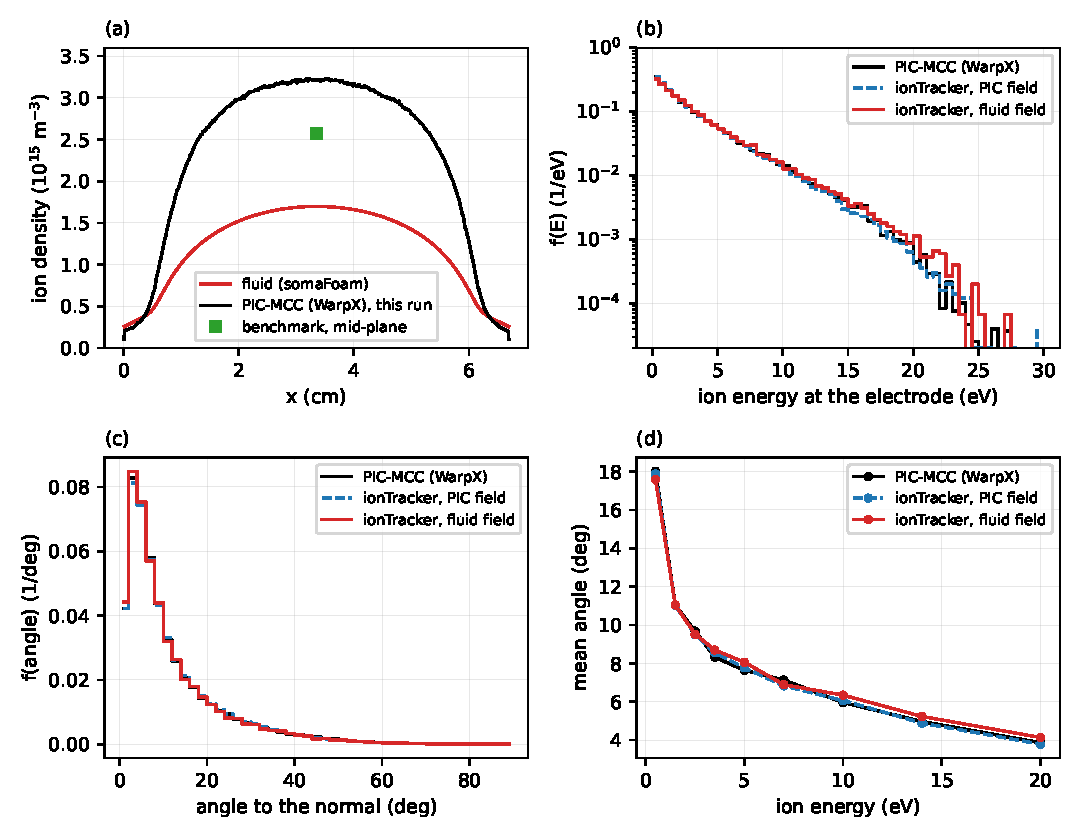
\includegraphics[width=0.86\textwidth]{fig_helium_comparison.pdf}
\caption{Example case. (a) Period-averaged ion density. (b) Energy and (c)
angular distributions of the He$^+$ ions at the electrodes. (d) Mean angle
against energy.}
\end{figure}

\begin{itemize}[leftmargin=1.4em,itemsep=1pt]
\item On the same field, \kw{ionTracker} and the particle-in-cell code agree
  within the statistical error of the histograms (about 1.4\,\%).
\item On the fluid field the energies are about 4\,\% higher (the
  period-averaged field at the wall is 22.0\,kV/m against 20.1\,kV/m), and
  the angles agree, although the density and the ion current of the fluid
  solution are far off: in this collisional sheath the distributions are set
  by the sheath field and the mean free path.
\item The ion flux, and with it the absolute scale of the distributions, is
  that of the fluid solution: 44\,\% too high here.
\item Both codes use the same model of ion--neutral scattering: the
  comparison does not test it.
\item For the run on the particle-in-cell field the profile of the ion source
  was estimated from the electrons at two phases of the period.
\end{itemize}

\textbf{Cost.} Step 1: 8\,s (3 threads). Step 2: about 6.5\,h on one core
(1.5 million time steps of 15\,ms, 256 cells). Step 3: 100\,000 ions in
6\,min on one thread; the tracked layer was 7\,mm thick. The
particle-in-cell runs took 16\,h each.

\section{What has been verified, and limits}

\begin{itemize}[leftmargin=1.4em,itemsep=1pt]
\item \kw{electronBoltzmann}: analytic distributions (constant cross
  section, constant collision frequency); the Monte Carlo method reproduces
  the Reid ramp benchmark.
\item \kw{ionTracker}: collisionless RF sheath against an independent
  integration; energy and angle with isotropic scattering in a uniform field
  against an independent Monte Carlo calculation; the Davis--Vanderslice
  distribution of a collisional sheath; ion mobilities in argon and helium.
\item \kw{ionTracker} against a particle-in-cell simulation of the example
  case, for the energy and angular distributions in a collisional RF sheath
  (section 8). The particle-in-cell run did not reproduce the bulk plasma of
  the benchmark; a comparison of the whole chain with a converged run is not
  available.
\item The ions follow the field of the fluid solution: an error of the fluid
  model in the sheath voltage or thickness goes into the distributions, and
  the ion flux is that of the fluid solution.
  Rates and transport against the local electron temperature are an
  approximation at low pressure, where the electrons are not in equilibrium
  with the local field.
\item Ion--neutral scattering is the sum of an isotropic and a backward
  (charge exchange) part. This reproduces ion transport; the wide-angle part
  of the angular distribution depends on this model.
\item The two-term solution treats ionisation as an energy loss and has no
  electron--electron collisions.
\item \kw{ionTracker} runs on one node (threads), on a static mesh, for one
  ion species; fast neutrals are not followed. The sheath launch has been
  run in one dimension only.
\end{itemize}

\end{document}
